\usepackage{listings}
\lstset{language=Python, showstringspaces=false}
\usepackage{graphicx}
\usepackage{tikz}
%\usepackage[a4paper,margin=1cm,landscape]{geometry}
\usetikzlibrary{positioning,shadows,arrows}

% $Header: /cvsroot/latex-beamer/latex-beamer/solutions/conference-talks/conference-ornate-20min.en.tex,v 1.7 2007/01/28 20:48:23 tantau Exp $

% This file is a solution template for:

% - Talk at a conference/colloquium.
% - Talk length is about 20min.
% - Style is ornate.



% Copyright 2004 by Till Tantau <tantau@users.sourceforge.net>.
%
% In principle, this file can be redistributed and/or modified under
% the terms of the GNU Public License, version 2.
%
% However, this file is supposed to be a template to be modified
% for your own needs. For this reason, if you use this file as a
% template and not specifically distribute it as part of a another
% package/program, I grant the extra permission to freely copy and
% modify this file as you see fit and even to delete this copyright
% notice. 


\mode<presentation>
{
  \usetheme{Warsaw}
  % or ...

  \setbeamercovered{transparent}
  % or whatever (possibly just delete it)
}


\usepackage[english]{babel}
% or whatever

\usepackage[latin1]{inputenc}
% or whatever

\usepackage{times}
\usepackage[T1]{fontenc}
% Or whatever. Note that the encoding and the font should match. If T1
% does not look nice, try deleting the line with the fontenc.


\title %[Short Paper Title] % (optional, use only with long paper titles)
{Obfuscating Python 3000}

%\subtitle
%{Include Only If Paper Has a Subtitle}

\author %[Author, Another] % (optional, use only with lots of authors)
{Andy Gurden} %F.~Author\inst{1} \and S.~Another\inst{2}}
% - Give the names in the same order as the appear in the paper.
% - Use the \inst{?} command only if the authors have different
%   affiliation.

\institute %[Universities of Somewhere and Elsewhere] % (optional, but mostly needed)
{
  Department of Computing\\
  Imperial College London
}
% - Use the \inst command only if there are several affiliations.
% - Keep it simple, no one is interested in your street address.

\date %[CFP 2003] % (optional, should be abbreviation of conference name)
{\today}
% - Either use conference name or its abbreviation.
% - Not really informative to the audience, more for people (including
%   yourself) who are reading the slides online

%\subject{Theoretical Computer Science}
% This is only inserted into the PDF information catalog. Can be left
% out. 



% If you have a file called "university-logo-filename.xxx", where xxx
% is a graphic format that can be processed by latex or pdflatex,
% resp., then you can add a logo as follows:

% \pgfdeclareimage[height=0.5cm]{university-logo}{university-logo-filename}
% \logo{\pgfuseimage{university-logo}}



% Delete this, if you do not want the table of contents to pop up at
% the beginning of each subsection:
%\AtBeginSubsection[]
%{
%  \begin{frame}<beamer>{Outline}
%    \tableofcontents[currentsection,currentsubsection]
%  \end{frame}
%}


% If you wish to uncover everything in a step-wise fashion, uncomment
% the following command: 

%\beamerdefaultoverlayspecification{<+->}


\begin{document}

\begin{frame}
  \titlepage
\noindent Supervised By: {Herbert Wiklicky}
\end{frame}

%\begin{frame}{Outline}
%  \tableofcontents
%  % You might wish to add the option [pausesections]
%\end{frame}


% Structuring a talk is a difficult task and the following structure
% may not be suitable. Here are some rules that apply for this
% solution: 

% - Exactly two or three sections (other than the summary).
% - At *most* three subsections per section.
% - Talk about 30s to 2min per frame. So there should be between about
%   15 and 30 frames, all told.

% - A conference audience is likely to know very little of what you
%   are going to talk about. So *simplify*!
% - In a 20min talk, getting the main ideas across is hard
%   enough. Leave out details, even if it means being less precise than
%   you think necessary.
% - If you omit details that are vital to the proof/implementation,
%   just say so once. Everybody will be happy with that.

Hello my name's Andy Gurden and I'm here to present my project - Obfuscating Python 3000. Before I even explain what this means,
I will describe to you the problem.

\section{Motivation}

\subsection{Why Obfuscate?}

\begin{frame}{Protecting Intellectual Property}
\begin{columns}[t]
\column{.5\textwidth}
  \begin{block}{Legal}
  \begin{itemize}
  \item Expensive
  \item Slow
  \item Difficult
  \item Not viable for smaller businesses
  \end{itemize}
  \end{block}

\pause

\column{.5\textwidth}
  \begin{block}{Technical}
  \begin{itemize}
  \item Often Cheap
  \item Can:
  \begin{itemize}
  \item Provide service only
  \item Encrypt code
  \item Distribute native code only
  \item<3> Obfuscate!
  \end{itemize}
  \end{itemize}
  \end{block}
\end{columns}
\end{frame}

If an individual or business puts hard work and time into creating software, they often have many techniques or algorithms that they worked hard to
develop. The last thing they want is for a reverse engineer to extract the juicy parts from their software, rebrand them and sell them for 2p cheaper.

There are a few ways it is possible to do this. We could use legal means, suing anyone we think has stolen our ideas, but this is expensive, slow, difficult
to prove and difficult to enforce, so is not really an option for general cases.

Alternatively we could use technical means which are often cheaper. The only sure-fire way to ensure parts of your software aren't stolen is to not give it out,
instead providing access as a service where all computation is performed server-side. Alternatively we could encrypt code, but this needs to be decrypted and run
in hardware to avoid a reverse engineer simply recording the code after a software decryption.

For languages such as Java or Python which are interpreted, we can compile to native machine code. This is much harder to reverse-engineer than the distributed formats
which are very simple to transform back to the original source code. Finally, and this is the reason we are all here, we could obfuscate the code.

\begin{frame}{What is Obfuscation?}
\begin{itemize}
\item ``Obfuscation is the concealment of intended meaning in communication, making communication confusing, intentionally ambiguous, and more difficult
      to interpret.'' \\ - Wikipedia
\end{itemize}
\begin{block}{Source Code Obfuscation}
Converting an existing program into a functionally identical equivalent that is harder to understand or reverse-engineer.
\end{block}
\begin{itemize}
\item Not completely safe
\item Automatic deobfuscators
\end{itemize}
\end{frame}

One of the first questions I usually get asked when talking about this project is, ''What the hell is obfuscation?``. Well we have the wikipedia version on the screen,
but in terms of software we want to modify our source program in such a way that it does the same things as it used to, just with very confusing source code.

This is not completely safe as we will still be handing our source over to the user, whom we do not entirely trust. Eventually with enough effort, someone will crack
the obfuscation, or 'deobfuscate' the program. The aim our obfuscation is then to make this task difficult enough for either a human or an automatic deobfuscator to
give up.

In Python, which we have taken as our target language, we distribute source code rather than bytecode or native code. So unless we create a service, obfuscating 
is really the only way to maintain portability and is a cheap and easy route to take.

\begin{frame}[fragile, label=pyobf_example]{Example of Obfuscated Code}
\begin{columns}[t]
\column{.5\textwidth}
\begin{block}{Plain Code}
\lstinputlisting[basicstyle=\scriptsize]{../snippets/beer.py.plain}
\end{block}
- PythonInfo Wiki

\pause

\column{.5\textwidth}
\begin{block}{Obfuscated Code}
\lstinputlisting[basicstyle=\scriptsize]{../snippets/beer.py.obf}
\end{block}
\end{columns}
\end{frame}

This is an example of some older Python code. After it has been run through an automatic obfuscator it is much harder to understand. Imagine a more complex example
and we can quickly see that a reverse engineer will have trouble following the code.

\subsection{Previous Work}

\begin{frame}<1>[label=current_solutions]{Current Solutions}
\begin{itemize}
\item Bytecode distribution
      \only<2->{
      \begin{itemize}
      \item Not secure
      \item Not portable
      \end{itemize}}
\item Implementing sensitive sections of code in C
      \only<3->{
      \begin{itemize}
      \item Much more secure
      \item Still not portable
      \end{itemize}}
\item pyobfuscate or other tools
      \only<4->{
      \begin{itemize}
      \item Moderate security
      \item Focus on layout obfuscation
      \item Outdated
      \end{itemize}}
\end{itemize}
\end{frame}

Currently solutions are to distribute bytecode, implement sections in C or use an automatic obfuscator. The example shows a flying pirate in disney's pirates of
the carribean online game. This is what happens when you distribute bytecode as it can be easily modified and turned back into source code. 

Implementing in C works, but just like bytecode it is not portable, relying on the user having CPython runtime and some architecture that you have compiled for.

We are left with pyofbuscate which was used to create the earlier example (show), and other tools online that do a similar job. These are few and far between, and have
not usually been updated recently meaning, their compatibility with newer versions of Python, in particular 3000 is not good. In fact pyobfuscate crashes if you
even try to run it on an interpreter newer than 2.6 (released in 2008).

In addition these tools tend to focus on layout obfuscation, rather than anything else, removing comments and scrambling identifier names. This is hard to read
but can be fixed easily a lot of the time by using an automatic deobfuscator.

\begin{frame}[plain]{Disney's Pirates of the Caribbean Online}
\resizebox{\textwidth}{!}{
\includegraphics{../images/POTC.eps}}
\end{frame}

\againframe<2-3>{current_solutions}

\againframe<2>{pyobf_example}

\againframe<4>{current_solutions}

% Talk about this when we create oat
%\begin{frame}{Other Types of Obfuscation}
%\begin{itemize}
%\item Talk about layout referring to pyobfuscate etc
%\item Talk about data
%\item Talk about control flow (examples)
%\end{itemize}
%\end{frame}

\section{Creating an Obfuscator}

\subsection{OAT - Obfuscation and Analysis Tool}

\begin{frame}{Presenting OAT - Obfuscation and Analysis Tool}
\begin{columns}
\column{0.5\textwidth}
\begin{itemize}
\item Interactive command line Python obfuscator
\item Performs control flow obfuscation on a program source, directed by the user.
\item Works on legal source code and produces legal source code.
\item Built for Python 3000.
\end{itemize}
\column{0.5\textwidth}
\resizebox{\textwidth}{!}{
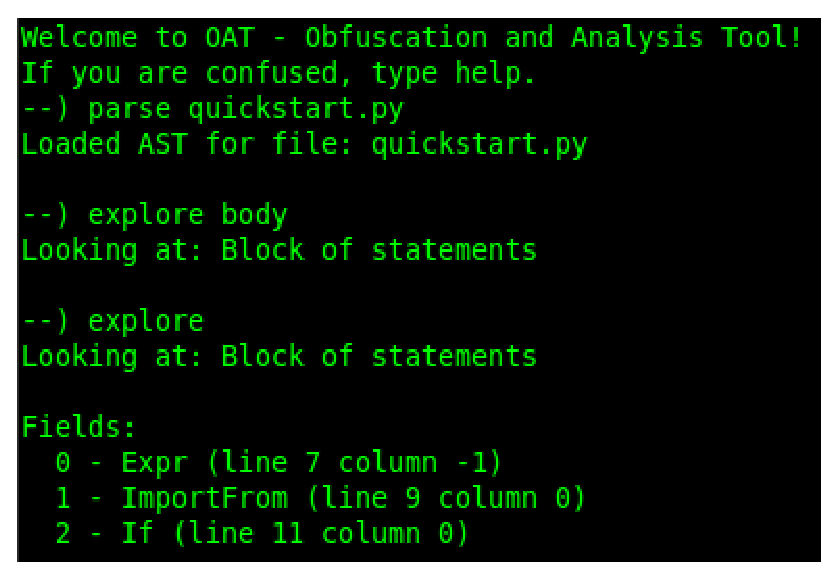
\includegraphics{../images/oat.eps}}
\end{columns}
\end{frame}

So we present our software, OAT - Obfuscation and Analysis Tool. This is a new interactive obfuscator that concentrates on control flow obfuscation.
This means that rather than altering layout of the source code, we try to change how the program actually runs, creating a confusing control flow while
keeping any results of the program the same.

Blah blah, 3000 so works on newer source code.

\begin{frame}<1>[label=workflow]{OAT Workflow}
\begin{itemize}
\item Parse a Python source file \visible<2->{- \alert<2>{Easy.}}
\item Analyse and mark the AST - Hard (3)
\item Program transformations - Depends on the transformation (4)
\item Output resulting source file \visible<3->{- \alert<3>{Simple idea. Takes time to cover entire language.}}
\end{itemize}
\end{frame}

From a user's perspective, the OAT workflow is very simple. We parse a file to receive an AST. Then analyse the tree for any information the program
transformations need. This is stored on the AST by 'marking' the nodes and avoids recalculating the same information again later.

The transformations can then be performed on the AST to create our new program. They will use our previous markings for all information that they will need.
Finally we will translate the AST back to a source file and print to screen or file.

\begin{frame}[fragile]{Parsing Source Files}
\begin{lstlisting}
import ast

with open("filename", "r") as file:
    ast.parse(file.read())
\end{lstlisting}

\vfill
This is Python. Python likes developers!
\end{frame}

Parsing can be done easily, this is Python after all.

\begin{frame}{Parsing Example}
Example from earlier, now written for Python 3.
\lstinputlisting[basicstyle=\small]{../snippets/beer.py.3}
\end{frame}

Now we can take a file, for example the code from earlier (now in Python 3) - notice print statement. By passing it though the code we get an AST.

\begin{frame}{Abstract Syntax Tree}
\begin{centering}
\scalebox{0.5}{
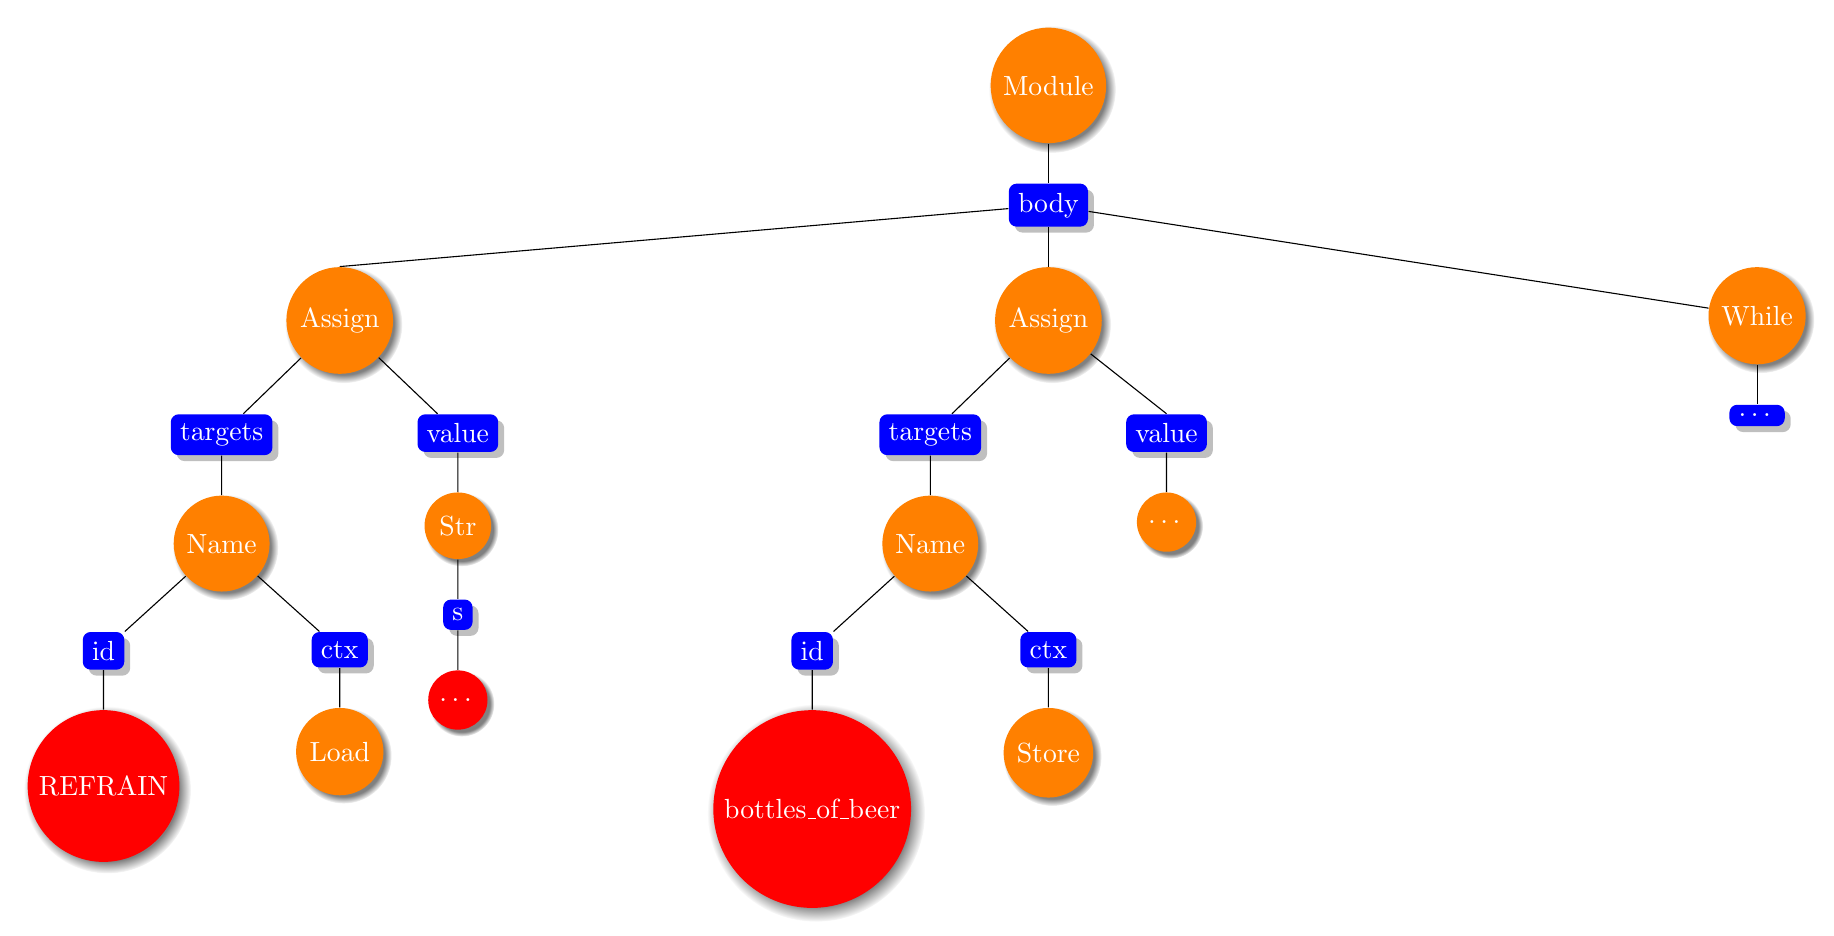
\begin{tikzpicture}[
    ast/.style={circle, draw=none, fill=orange, circular drop shadow,
        text centered, anchor=north, text=white},
    field/.style={rectangle, draw=none, rounded corners=1mm, fill=blue, drop shadow,
        text centered, anchor=north, text=white},
    value/.style={circle, draw=none, fill=red, circular drop shadow,
        text centered, anchor=north, text=white},
    level distance=0.5cm, growth parent anchor=south
]
\node (Module) [ast] {Module} 
    child{ [sibling distance=9cm]
        node (ModuleBody) [field] {body}
        child{ [sibling distance=3cm]
            node (Assign) [ast] {Assign}
            child{
                node (assigntargets) [field] {targets}
                child{
                    node (name) [ast] {Name}
                    child{
                        node (id) [field] {id}
                        child{
                            node (nm) [value] {REFRAIN}
                        }
                    }
                    child{
                        node (ctx) [field] {ctx}
                        child{
                            node (ctxl) [ast] {Load}
                        }
                    }
                }
            }
            child{
                node (assignvalue) [field] {value}
                child{
                    node (Str) [ast] {Str}
                    child{
                       node (strs) [field] {s}
                       child{
                            node (strval) [value] {\ldots}
                        }
                    }
                }
            }
        }
        child{ [sibling distance=3cm]
            node (Assign) [ast] {Assign}
            child{
                node (asstarg) [field] {targets}
                child{
                    node (tname) [ast] {Name}
                    child{
                        node (tnameid) [field] {id}
                        child{
                            node (tnameidb) [value] {bottles\_of\_beer}
                        }
                    }
                    child{
                        node (tnamectx) [field] {ctx}
                        child{
                            node (tnamectxs) [ast] {Store}
                        }
                    }
                }
            }
            child{ [sibling distance=3cm]
                node (asgtiji) [field] {value}
                child{
                    node (asf) [ast] {\ldots}
                }
            }
        }
        child{
            node (While) [ast] {While}
            child{
                node (gte) [field] {\ldots}
            }
        }
    }
;
\end{tikzpicture}}
\end{centering}
\end{frame}

We receive an AST, something like this unfinished specimen.

\againframe<2>{workflow}

We will look next at printing a source file.

\begin{frame}[fragile]{Design of a Source Writer}
\begin{itemize}
\item In-order traversal of the AST
\item Separate method to print each possible node type
\item Slow to implement initially
\item Quick and easy to extend for different coding styles
\end{itemize}

\begin{lstlisting}
if 1 < 2:
    print("Hello World")
\end{lstlisting}
\end{frame}

\begin{frame}<-14>[fragile]{Source Writer Example}
\begin{columns}[b]
\column{.5\textwidth}
{\small
\begin{semiverbatim}
\alert<2-13>{Module}
\alert<2-13>{  - body: If}
\alert<3-5>{    - test: Compare}
\alert<3>{      - left: Num}
\alert<3>{        - n: 1}
\alert<4>{      - ops: Lt}
\alert<5>{      - comparators: Num}
\alert<5>{        - n: 2}
\alert<7-13>{    - body: Expr}
\alert<7-13>{      - value: Call}
\alert<7-8>{        - func: Name}
\alert<7>{          - id: 'print'}
\alert<8>{          - ctx: Load}
\alert<10-12>{        - args: Str}
\alert<11>{          - s: 'Hello World'}
\end{semiverbatim}}
\column{.5\textwidth}
\begin{semiverbatim}
\textbf{
\uncover<2->{if }\uncover<3->{1} \uncover<4->{<} \uncover<5->{2}\uncover<6->{:}
\quad\quad\uncover<7->{print}\uncover<9->{(}\uncover<10->{"}\uncover<11->{Hello World}\uncover<12->{"}\uncover<13->{)}
}
\end{semiverbatim}
\end{columns}
\end{frame}

\againframe<3>{workflow}

(explain because python does not need this to run, it does not do it)
\subsection{Basic Ideas for Proofs/Implementation}

\begin{frame}{Make Titles Informative.}
\end{frame}

\begin{frame}{Make Titles Informative.}
\end{frame}

\begin{frame}{Make Titles Informative.}
\end{frame}



\section*{Summary}

\begin{frame}{Summary}

  % Keep the summary *very short*.
  \begin{itemize}
  \item
    The \alert{first main message} of your talk in one or two lines.
  \item
    The \alert{second main message} of your talk in one or two lines.
  \item
    Perhaps a \alert{third message}, but not more than that.
  \end{itemize}
  
  % The following outlook is optional.
  \vskip0pt plus.5fill
  \begin{itemize}
  \item
    Outlook
    \begin{itemize}
    \item
      Something you haven't solved.
    \item
      Something else you haven't solved.
    \end{itemize}
  \end{itemize}
\end{frame}



% All of the following is optional and typically not needed. 
\appendix
\section<presentation>*{\appendixname}
\subsection<presentation>*{For Further Reading}

\begin{frame}[allowframebreaks]
  \frametitle<presentation>{For Further Reading}
    
  \begin{thebibliography}{10}
    
  \beamertemplatebookbibitems
  % Start with overview books.

  \bibitem{Author1990}
    A.~Author.
    \newblock {\em Handbook of Everything}.
    \newblock Some Press, 1990.
 
    
  \beamertemplatearticlebibitems
  % Followed by interesting articles. Keep the list short. 

  \bibitem{Someone2000}
    S.~Someone.
    \newblock On this and that.
    \newblock {\em Journal of This and That}, 2(1):50--100,
    2000.
  \end{thebibliography}
\end{frame}

\end{document}


